\chapter{Grundlagen}

In diesem Kapitel werden die theoetischen Grundlagen für diese Arbeit aufgezeigt und Beschrieben. 

\section{arUco Marker}\label{arucoMarker}

arUco Marker sinnd quadratische systhetische Marker, bestehend aus einem schwarzen Rand und einer binären Matrix, dessen quadratische 
Elemente in proportional zu der Dicke des schwarzen Rands stehen. Die binäre Matrix kann zu einem Integerwert decodiert werden, welche
als ID genutzt werden kann, dabei wird die Binärmatrix jedoch nicht als Binärzahl dekodiert, sondern die Marker sind ihrem Platz im Dictionary ihres Typs aufsteigend zugeordnet.
Der Erkennungsalgorhitmus nutzt Graustufenbilder und gilt als robust. 
Er beruht zunächst auf der Erkennung rechteckiger Merkmale. 
Die detektierten Bildbereiche werden anschließend in ein binäres Bild transformiert und perspektivisch entzerrt. 
Anschlißend werden die Marker mit einer vordefinierten Maske dekodiert.
Die Größe der Matrix wird dabei aus dem Markertyp und der Breite des schwarzen Rands berechnet.
Im Standardfall entspricht die Breite des Rands genau der Pixelbreite und -Höhe von einem Bit. 
Neben der ID werden dabei auch die Ecken der Marker erkannt und die Lage im Originalbild gespeichert. 
ID's und Markerecken sind die wichtigsten Rückgabewerte des Algorhythmus.
Merkmale im Bild, die im Verlauf der Algorhythmus als Marker abgelehnt werden, werden als drittes Rückgabeargument zurückgegeben.
Im Quellcode der Software sind diese stets als \verb|ids|, \verb|corners| und \verb|rejected| bezeichnet.

Durch die Lokalisierung der Ecken im Originalbild können arUco Marker gut für Aufgaben wie Kamerakalibrierung, Objektlokalisierung, Abstandsmessung sowie Roboternavigation genutzt werden.
\cite[OpenCV arUco]{OpenCVaruco}
Durch die vorgefertigte Maske ist die Erkennung immer an ein Dictionary des verwendeten Markers gebunden. 
Wichtigstes Merkmal ist dabei die Größe der Binärmatrix. In dieser Arbeit werden Marker des Typs 6x6-250 verwendet.
Dabei steht 6x6 für die Größe der Binärmatrix in Bits und 250 steht für die Anzahl der Pixel.

\begin{figure}
    \caption{Beispiel für eine erfolgreiche Erkennung von arUco Markern. Quelle: \cite[OpenCV]{OpenCVaruco}}\label{fig:aruco1}
    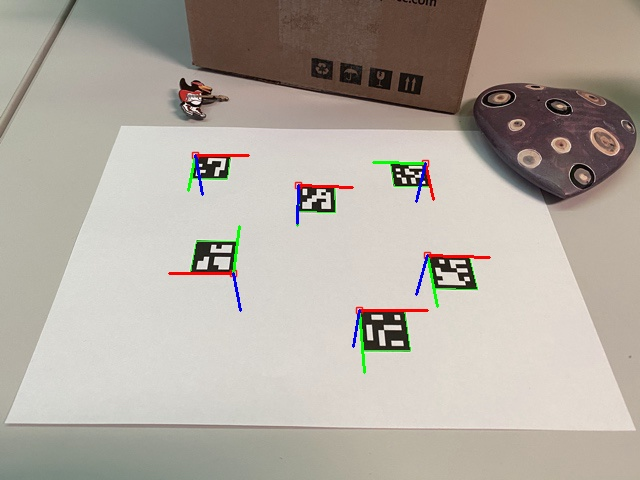
\includegraphics[width = \textwidth/2]{Bilder/singlemarkersaxes.jpg}
    \centering
\end{figure}

\begin{figure}
    \caption{Bild nach Graustufenumwandlung und Umwandlung in Binärbild. Quelle: \cite[OpenCV]{OpenCVaruco}}\label{fig:aruco2}
    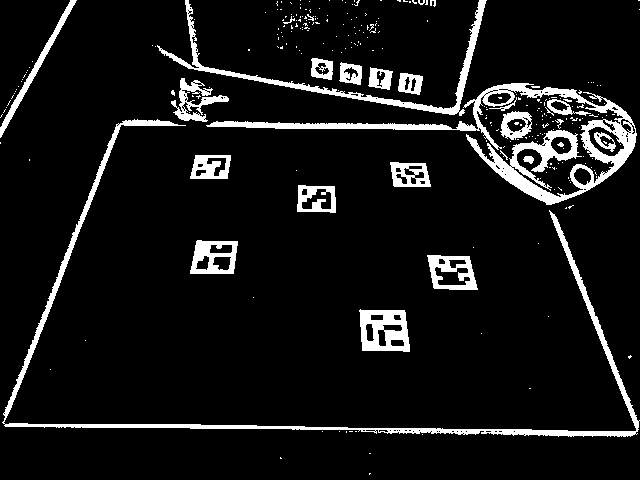
\includegraphics[width = \textwidth /2]{Bilder/singlemarkersthresh.png}
    \centering
\end{figure}

\subsection{Erkennungsalgorhitmus}
Die Erkennung der Marker erfolgt in den nachfolgenden Schritten: 

\begin{enumerate}
    \item Einlesen des Bildes, z.B. \ref{fig:aruco1}
    \item Umwandeln des Bilds in ein Graustufenbild 
    \item Umwandeln des Bilds in ein Binärbild \ref{fig:aruco2}
    \item Erkennen rechteckiger Merkmale
    \item Rectifizierung der Merkmale \ref{fig:aruco4}
    \item Bitextraktion der Binärmatrix (Bilder \ref{fig:aruco5} \ref{fig:aruco6})
    \item Decodierung der Binärmatrix ergibt die ID und Ecken des Markers
\end{enumerate}

Bei der Umwandlung in ein Binärbild kann der Erkennungsalgorithmus schon fehlschlagen. Die Gründe dafür werden im Kapitel \ref{KameragestützteInventur}
behandelt.

\begin{figure}
    \caption{Beispiel für eine fehlgeschlagene Umwandlung in ein Binärbild. Dieser Marker würde nicht erkannt. Quelle: \cite[OpenCV]{OpenCVaruco}}\label{fig:aruco3}
    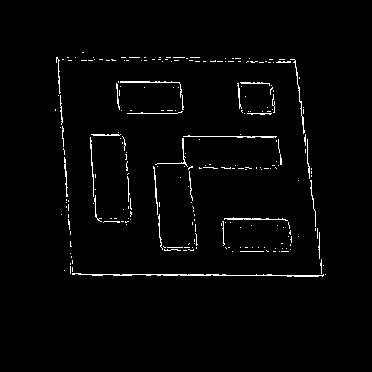
\includegraphics[width = \textwidth/2]{Bilder/singlemarkersbrokenthresh.png}
    \centering
\end{figure}

Anschließend werden rechteckige Merkmale gesucht und diese Rektifiziert \ref{fig:aruco4}. 

\begin{figure}
    \caption{Rektifizierung eines extrahierten Markers. Quelle: \cite[OpenCV]{OpenCVaruco}}\label{fig:aruco4}
    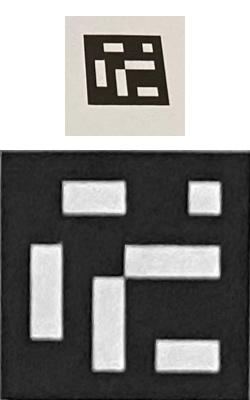
\includegraphics[width = \textwidth/3]{Bilder/removeperspective.jpg}
    \centering
\end{figure}

\begin{figure}
    \caption{Bitextraktion der Binärmatrix. Quelle: \cite[OpenCV]{OpenCVaruco}}\label{fig:aruco5}
    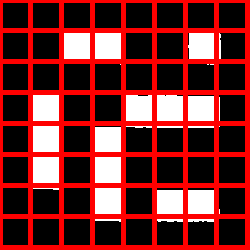
\includegraphics{Bilder/bitsextraction1.png}
    \centering
\end{figure}

\begin{figure}
    \caption{Bitextraktion der Binärmatrix. Quelle: \cite[OpenCV]{OpenCVaruco}}\label{fig:aruco6}
    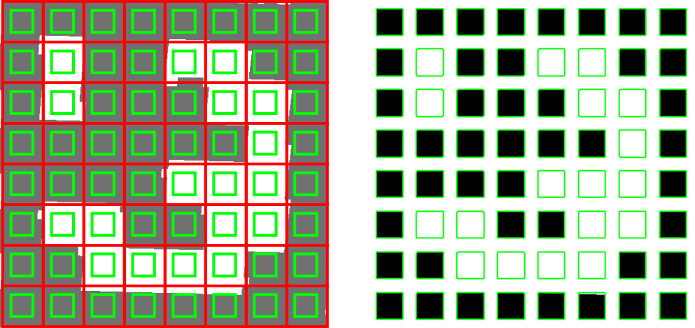
\includegraphics[width = \textwidth]{Bilder/bitsextraction2.png}
    \centering
\end{figure}



\section{Grundlagen der Softwarearchitektur}

Die in dieser Arbeit verwendeten Grundlagen zur Softwarearchitektur beschränken sich auf den Kurs "Programmierung und Modellierung" des Fachbereichs
FB16 der Universität Kassel. Der Inhalt reicht von dem Erstellen von textuellen Szenarien einer Software, über die Konzeptionierung von GUIs bis hin
zu den Grundlagend der Servertechnik am Beispiel des REST Protokolls und websockets. 
Der größte Thementeil ist jedoch die Modellierung von Datenmodellen und ihre referenzielle Integrität, welches im Zusammenhang mit UML-Diagrammen gelernt wurde.
Referenzielle Integrität von Datenmodellen spielt in Python eine eher untergeordnete Rolle, da es keine privaten oder geschützten klassenattribute gibt. 
Dennoch bietet ihre Verwendung eine gute Möglichkeit, um die Datenmodelle in ihrer gewohnten Komplexizität zu gestalten, die
Verwendung jedoch einfach zu halten.

\section{OPC UA}

OPC UA ist ein offener Standard für die Kommunikation zwischen Maschinen der \cite[OPC Foundation]{OPCFoundation}. Es ist ein schlankes Protokoll, 
welches verschlüsselte Übermittlung von Maschineninformationen, Sensordaten, Prozessdaten und anderen Daten ermöglicht.
OPC UA ist ein wichtiger Bestandteil des Programms Industrie 4.0. 
Üblichwerweise sind alle Ebenen Prozessteuerungspyramide eingebunden, die von SPSen bis hin zur Geschäftsleitung reichen kann.

Für diese Arbeit gibt es im Wesentlichen zwei Möglichkeiten das OPC UA Protokoll zu benutzen. 
Zum Einen bietet das \cite[Qt Framework]{QtOPCUA} eine Implementierung des Protokolls. 
Zum Anderen gibt es ein offenes GitHub Repository \cite[FreeOpcUa]{asyncua}, das als Python Paket zur Verfügung steht. 
Da in anderen Python Programmen der $\mu$Plant bereits FreeOpcUa verwendet wird, wird diese Bibliothek auch in dieser Arbeit verwendet.
Das erleichtert die Integration der OPC UA Funktionalität in die $\mu$Plant und eine zukünftige Wartung und Erweiterung der Software.

Während der Entwicklung der Software wurden zu testzwecken zwei Programme verwendet um die erstellten Server zu testen. 
Für Windows wurde der \cite[OPC UA Client UaExpert]{UaExpert}verwendet. Da ich jedoch unterwegs auf MacOS programmiere wurde 
ein OPC UA Client \cite[OPC UA Client für Mac]{uaClientMac} verwendet. 
Dieser hat zwar nicht den gleichen Funktionsumfang, ist aber dennoch für Debug-Zwecke nützlich. 

\section{RFID Technologie}

Laut der Website \cite[RFID Grundlagen]{RFIDGrundlagen} sind die Anfänge der RFID Technologie bis in den zweiten Weltkrieg zurückzuführen, 
in dem eine Art sekundärradar zur Feinerkennung eingesetzt wurde. Als Begründer der heutigen RFID Technologie gilt der Schwede Harry Stockman. 
Bei der Technologie handelt es sich um ein System zur Kontaktlosen Informationsübermittlung (lesen und schreiben). 
Dazu wird in der Regel ein Transponder und ein Lesegerät benötigt. Beide Einheiten fügen über ausgeprägte Antennen.
Das Lesegerät erzeugt ein elektromagnetisches Feld, welches einerseits zur Spannungsversorgung des IC des Transponders genutzt wird.
Gleichzeitig dient das Feld als Taktgeber und zur Informationsübermittlung. 
Während das Lesegerät nicht sendet, kann der Transponder Daten übermitteln. 
Für die Transponder gibt es verschiedene Standards auf die im Rahmen dieser Arbeit nicht weiter eingegangen werden. 
Die Daten auf dem Transponder sind in Blöcke aufgeteilt, die jeweils eine bestimmte Anzahl an Bytes enthalten.
Je Transponder ist ein Block für eine UID reserviert, die im Allgemeinen nicht verändert werden kann.

In der $\mu$Plant werden Lesegeräte der Firma \cite[FEIG GmbH]{RFIDFeig} vom Typ ID ISC.MRU102-PoE-LED verwendet. 
Die Lesegeräte sind in jeder Station der $\mu$Plant verbaut.
Die Transponder sind jeweils auf der Rückseite eines jeden Bechers aufgeklebt. 
Jedem Becher ist somit eine eigene UID zugeordnet. Die Datenübertragung der LEsegeräte erfolgt über TCP/IP.
Die Firma Feig stellt ein umfassendes SDK zur Verfügung, bietet jedoch keinen Python Support.


\section{Die Programmiersprache Python}

Python ist eine universelle, interpretierte Hochsprache. Der Programmcode kommt dabei ohne Klammer und Semikolons aus.
Die Formatierung des Codes erfolgt über Einrückungen. \cite[Python]{Python} ist leicht zu lernen, intuitiv zu nutzen und unterstützt die 
meisten Programmierparadigmem wie Objektorientierung, funktionale Programmierung und aspektorientierte Programmierung. 

Die Version, die in dieser Arbeit verwendet wird, ist Python 3.11 - was zu Beginn dieser Arbeit die neueste Version war. 

\section{Die Programmiersprache C++}

C++ ist eine universelle, kompilierte Hochsprache. Sie ist eine Weiterentwicklung der Programmiersprache C und unterstützt die
Programmierparadigmen Objektorientierung, generische Programmierung und prozedurale Programmierung.
Der Standard ist sehr Komplex und besteht aus mehreren Teilen, die an und für sich eigenständig anwendbar aber auch kombinierbar sind.

In dieser Arbeit wird C++ in der Version 23 verwendet um das SDK der Firma Feig zu zu nutzen und ausschließlich die gewünschten Funktionen 
in Python mit dem Python Paket ctypes zu verwenden.

Auch für das Legacy Framework ABB Robotics wird C++ verwendet um das Framework für Python nutzbar zu machen.
Die Programme sind dabei in Visual Studio 2019 erstellt und Kompiliert worden. 

\section{Die Programmiersprache C\#}\label{Csharp}

C$\#$ ist eine Komponentenorientierte Programmiersprache und historisch die Antwort auf die von SUN veröffentlichte Sprache Java. 
Sie wird häufig mit dem .NET Framework verwendet - so auch in der Software Lagerverwaltung 3.0 welche in meiner \cite[Semesterarbeit]{Semesterarbeit}
Grundlage für die Konzeptionierung der neuen lagersoftware war. 
Das GUI wird dabei in .xaml Dateien in einer Modellierungssprache erstellt - meistens mit einem Integrierten Editor. Der Controller code für die GUI-Elemente 
findet sich in einer xaml.cs Datei. Zusammen mit dem Code für die Geschäftslogik ist Software, die in C$\#$ geschrieben ist, oft nicht leicht zu überschauen. 
Daher sind Teile der Software Lagerverwaltung 3.0 in dieser Arbeit nur prinzipiell unter visuellen (GUI) und funktionellen Aspekten übernommen worden.

\section{Das Qt Framework}

Laut der \cite[Qt Wiki Website]{qtWikiHistory} wurde das Qt Framework geboren, als ihre Schöpfer Haa-
vard Nord und Eric Chambe-Eng im Sommer 1990 in Norwegen an einem GUI für eine
Ultraschalldatenbank arbeiteten. Die Software sollte damals in C++ implementiert auf
Mac, Unix und Windows laufen. Fünf Jahre später veröffentlichten Sie das erste Qt Fra-
mework unter dem Firmennamen Troll Tech. Seitdem gewann das Framework immer
mehr Popularität. Im Jahr 2006 übernahm Nokia die Firma Troll Tech und verkaufte das
Qt Project in den Jahren 2011 und 2012 erst teilweise, dann vollständig an den Digia
Konzern. Seit 2014 ist Qt als Tochterunternehmen des Digia Konzerns unter dem Namen
„The Qt Company“ ein eigenständiges Unternehmen.
Das Qt Framework ist in C++ implementiert.

\subsection{PySide6 Bindings}

Für die Programmiersprache wurden hostorisch zwei Frameworks veröffentlicht. Die Firma Riverbank veröffentlichte für das Qt4 die Bindings PyQt4.
Die Bindings sind sehr eng an der C++ Implementierung des Qt Frameworks orientiert.
Die Firma Nokia hat ebenfalls die PySide Bindings veröffentlicht, die mehr an der Python Syntax orientiert sind.
The Qt Company hat das PySide Framework übernommen und weiterentwickelt. 
Beide Frameworks sind sowohl mit kommerziellen als auch mit Open Source Lizenzen verfügbar.
Im Jahr 2023 wurde das PySide6 Framework für Qt6 veröffentlicht welches nun auch QtQuick und QML voll unterstützt. 
Bei dem PySide6 Framework handelt es sich um automatisch generierte Bindings für das Qt Framework. 
Das Qt Framework in der C++ Implementierung muss daher immer mit installiert werden. 
Leider sind bei der automatischen Generierung der Bindings keine Dokumentationen entstanden.
Eine dauernde, parallele Recherche in der Qt Dokumentation ist daher unerlässlich und verleitet dazu eine gleichartige
Programmierweise zu entwickeln und sich auf bekannte Strukturen zu verlassen.

\subsection{QtQuick 2.0 und QML}

Neben herkömmlichen Entwicklung für GUIS mittels Widgets,  bietet das Qt Framework auch die Möglichkeit, GUIs mit QML zu erstellen.
QML und XAML (siehe \ref{Csharp}) sind beide deklarative Sprachen, in denen GUIs oder ihre Elemtente in einer Datei gespeichert,
dessen Format an das XML Format angelehnt ist.
Im Vergleich zu XAML ist QML leichter lesbar und besser strukturiert, was auf seinen leicht verständlichen Javascript-Syntax zurückzuführen ist.
Einfache GUI Elemeente lassen sich dadurch auch ohne Editor erstellen.
GUI Inhalte werden durch die Klasse \verb|QtQMLApplicationEngine| in Python geladen und gerendert. 
Eine Besonderheit der Sprache QML ist, dass sie JavaScript unterstützt. Es ist somit möglich funktionalen Code in einer QML Datei zu schreiben. 
Die Ausführung des Javascript Codes kann jedoch zu Performance Problemen führen. 
Deshalb empfiehlt es sich nicht große Teile des Backends in QML zu implementieren.

QtQuick 2.0 ist eine Standardbibliothek in Qt, die grundlegende QML Types enthält, z.B, ein Knopf oder eine Listenanicht.
Der Softwareentwickler kann diese Typen beliebig kombinieren und die Kombinationen dann als eigene Typen abspeichern. 
So lassen sich leicht komplexe und dynamische GUIs erstellen. 
Da neben der GUI Modellierung trotzdem ein Python Backend für die Geschäftslogik und die Verbindung des GUIs zur Datenquelle benötigt wird 
und QML für das Rendern schon Datentypen enthält, die das Rendern von Datenmodellen erleichtern, 
eignet sich QtQuick 2.0 besonders gut für die Umsetzung des MVVC Design-Konzept der Softwareentwicklung.
Die QML-Datentypen wie z.B. \verb|QAbstractListModel| sind dabei als viewmodel zu verstehen. Der gerenderte Inhalt ist die view.
Die Controller sind in dieser Arbeit als eigenständige Python Module implementiert.
Für Listen und Tabellenansichten sei angemerkt, dass in der Regel neben der eigentlichen Listenansicht auch ein QML Type für das Delegate 
erstellt werden muss - Also ein GUI Element, das festlegt wie der einzelne Listeneintrag aussehen soll.